\section{Att tolka andragradsuttryck}

Ekvationer för räta linjer kan skrivas på en rad olika sätt -- ekvationerna $y = -2x + 3$, $y + 2x = 3$ och $y + 2x - 3 = 0$ beskriver alla samma linje.
Beroende på hur man skriver ekvationen går det lättare eller svårare att läsa av olika egenskaper för linjen, som lutning eller skärning med y-axeln.

Precis som räta linjer, kan andragradsfunktioner skrivas på ett antal olika sätt.
Det sätt man vanligtvis ser är \mbox{$f(x) = ax^2 + bx + c$}, exempelvis $y=2x^2 - 12x + 19$, men vi kommer till en början att fokusera på formen \mbox{$f(x) = a(x+d)^2+e$} istället -- exempelvis $y=2(x-3)^2+1$.

Det sättet att skriva andragradsuttryck på kallas \emph{kvadratkompletterad form} (eftersom uttrycket består av en kvadrat som kompletterats med en konstant).
Om en andragradsfunktion är skriven på kvadratkompletterad form är det lätt att hitta extrempunkter och extremvärden för funktionen, och det går också relativt lätt att lösa ekvationer som består av kvadratkompletterade andragradsuttryck.

\subsection{Hitta extremvärdet för en andragradsfunktion}

\begin{figure}
  \centering
  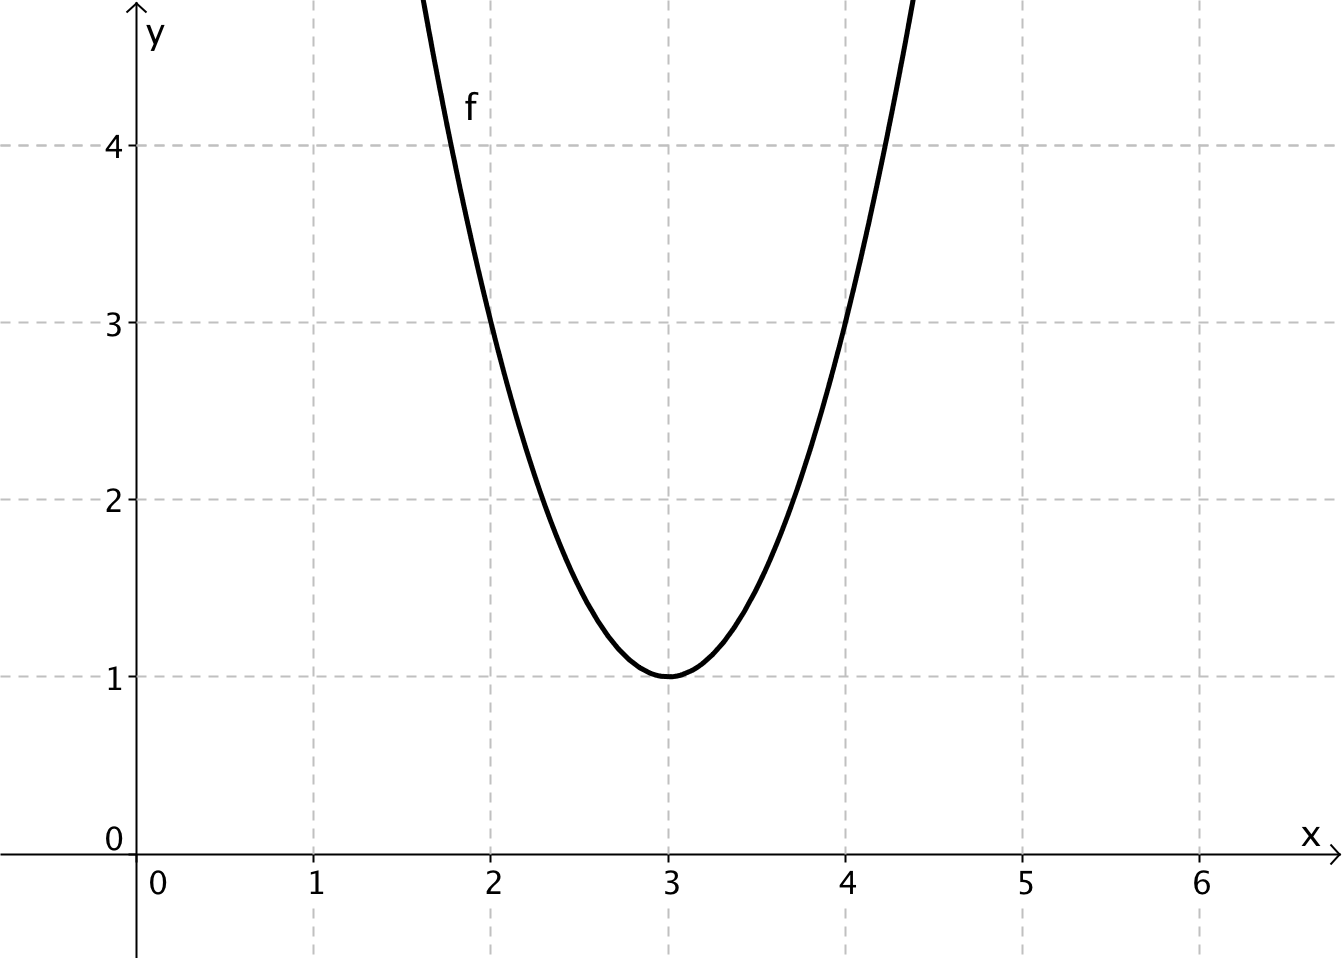
\includegraphics[width=0.7\textwidth]{bilder/poskurva1.png}
  \caption{\label{fig:poskurva1}Grafen till funktionen $f(x)=2(x-3)^2+1$.}
\end{figure}

Ta en titt på grafen till funktionen $f(x) = 2(x-3)^2+1$.
Vi kan se från funktionens graf att det minsta värdet funktionen kan anta är 1, och vi kan se att det värdet får funktionen när $x=3$.
Men vi kan läsa samma information direkt ur funktionsuttrycket också. Hur då?

Funktionsuttrycket består av två delar -- en kvadrat $2(x-3)^2$ vars värde bestäms av $x$, och en konstant 1.
Beroende på vilket värde vi ger $x$ kommer kvadratdelen att bli olika stor, men den kommer alltid att bli \emph{positiv} (eftersom även negativa värden blir positiva när de kvadreras).
Vi skulle alltså kunna tolka funktionen som att vi har talet 1, och ska lägga till ett annat tal som är 0 eller större beorende på vad x är.

Ser man funktionsuttrycket på det viset är det ganska lätt att se att 1 är det minsta värdet som funktionen kan ha.
Vi kan i allmänhet dra slutsatsen att om en andragradsfunktion beskrivs av $f(x)=a(x+d)^2+e$ är funktionens extremvärde $e$.

Om vi inte bara är intresserade av extrevärdet, utan även \emph{extrempunkten}, räcker det inte att hitta y-värdet för extrempunkten -- vi måste också hitta vilket x-värde som ger funktionen dess extremvärde.
När blir $f(x) = 2(x-3)^2+1$ så litet som möjligt?
Ja, om funktionen består av talet 1 plus en kvadratterm, måste funktion få sitt lägsta värde när kvadraten är noll.
När blir $2(x-3)^2 = 0$? Jo, när värdet inomparentes blir noll -- det vill säga när $x = 3$.
Vi kan i allmänhet dra slutsatsen att om en andragradsfunktion beskrivs av $f(x)=a(x+d)^2+e$ är x-koordinaten för funktionens extrempunkt $-d$.

\subsubsection{Positiva och negativa andragradsfunktioner}

\begin{figure}
  \centering
  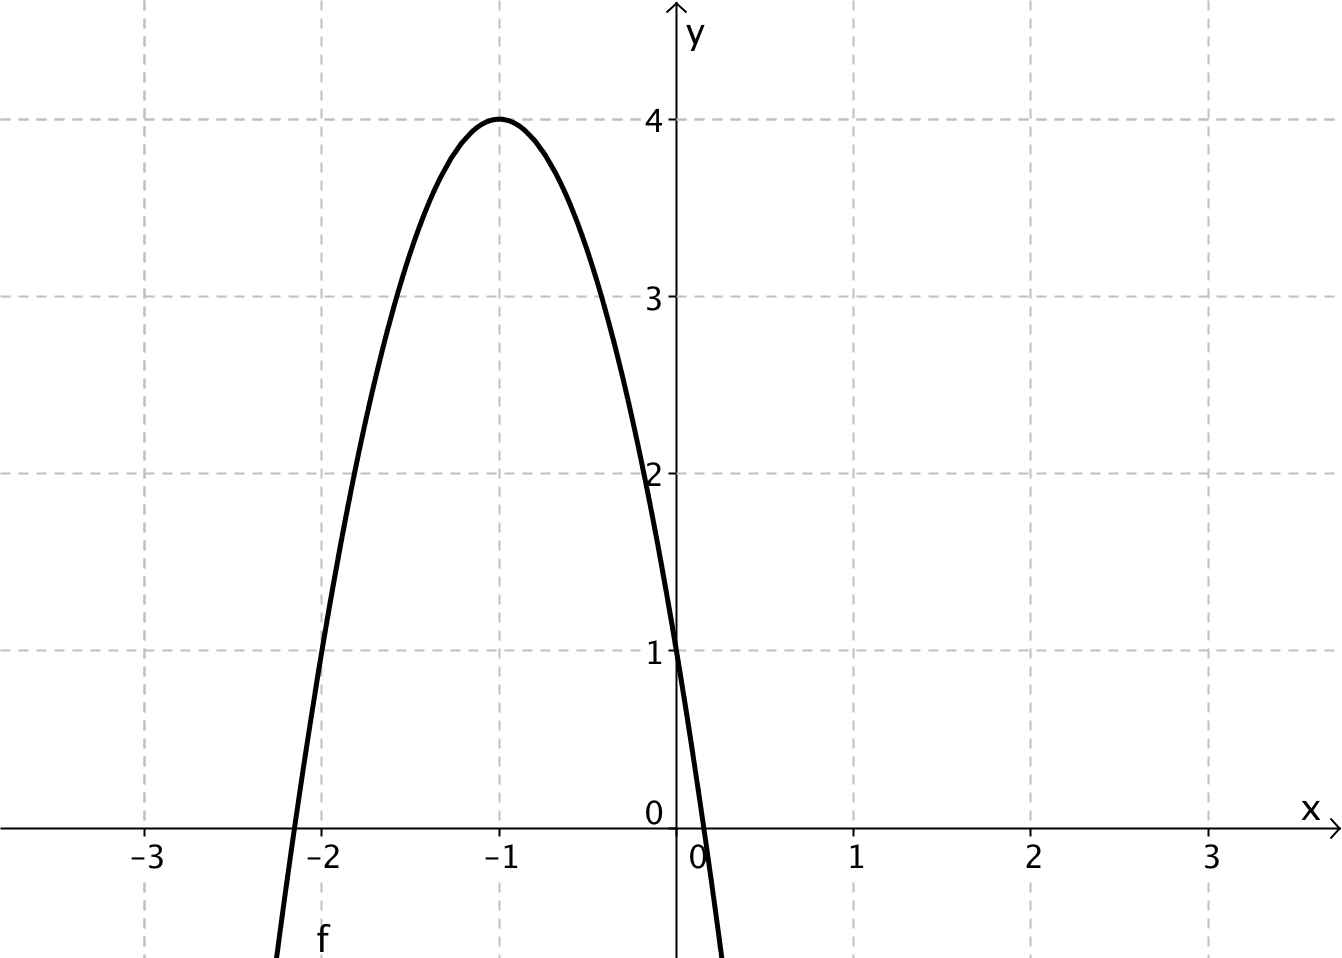
\includegraphics[width=0.7\textwidth]{bilder/negkurva1.png}
  \caption{\label{fig:negkurva1}Grafen till funktionen $f(x)=-3(x+1)^2+4$.}
\end{figure}

I den här grafen syns en annan andragradsfunktion, nämligen $f(x)=-3(x+1)^2+4$.
Vi kan, både från grafen och funktionsuttrycket, se att funktionens extrempunkt är $(-1, 4)$.
Men extrempunkten är en \emph{maximumpunkt} -- den högsta punkten på kurvan -- istället för en minimumpunkt.

Även detta kan vi läsa direkt från funktionsuttrycket:
Kvadrattermen är i det här fallet \emph{negativ}; i förra exemplet hade vi ``1 plus en kvadrat'', men här har vi istället ``4 \emph{minus} en kvadrat''.
Funktionens värde kommer alltså att vara \emph{som mest} 4, och det värdet får funktionen då kvadraten blir noll (det vill säga $x=-1$).

Vi kan i allmänhet dra slutsatsen att om faktorn $a$ är positiv har funktionen en minimumpunkt, och om $a$ är negativ har funktionen en maximumpunkt.
Man brukar ibland prata om positiva och negativa andragradsfunktioner, vilket betyder att $a$-värdet är positivt eller negativt.

\subsection{Symmetrilinje}



\subsection{Sammanfattade termer och uttryck}

\begin{itemize}
  \item Andragradsuttryck på allmän form: $ax^2+bx+c$
  \item Andragradsuttryck på kvadratkompletterad form: $a(x+d)^2+e$
  \item En andragradsfunktion $f(x)=a(x+d)^2+e$ har extremvärdet $e$.
  \item En andragradsfunktion $f(x)=a(x+d)^2+e$ har extrempunkten $(-d, e)$.
  \item $a > 0$ betyder att funktionen har en minimumpunkt (och är en positiv andragradsfunktion).
  \item $a < 0$ betyder att funktionen har en maximumpunkt (och är en negativ andragradsfunktion).
\end{itemize}

\subsection{Uppgifter och övningar}

(Bara skisser än så länge.)

\begin{enumerate}[label=\bfseries Uppgift \thechapter . \arabic*:]
  \item \url{http://www.geogebratube.org/student/m115801}
  \item Beskriv i ord vad skillnaden mellan ett extremvärde och en extrempunkt är.
  \item Förklara i ord vad en maximumpunkt och en minimumpunkt är, och hur man kan avgöra om en andragradsfunktion har en max- eller minpunkt.
  \item \emph{Måste} alla andragradsfunktioner ha en extrempunkt? Försök att hitta ett undantag.
  \item Vad är extremvärdet och extrempunkten för funktionerna i de här graferna?
  \item Vad är extremvärdet och extrempunkten för de här funktionsuttrycken?
  \item Den här grafen föreställer funktionen $f(x)=1{,}5(x+d)^2+e$. Vad är värdet på $d$ och $e$?
  \item Den här grafen föreställer funktionen $f(x)=a(x+d)^2+e$. Är $a$ positivt eller negativt?
  \item Skissa grafen till funktionen $f(x)=-2(x+1)^2-3$.
  Börja med att skissa utan att räkna ut några funktionsvärden, och testa sedan att räkna ut några punkter på grafen och se hur bra skissen stämmer.
  \item När värdet på $e$ ökar flyttas grafen för $f(x)=a(x+d)^2+e$ längre upp. Förklara varför!
  \item När värdet på $d$ ökar flyttas grafen för $f(x)=a(x+d)^2+e$ längre åt vänster. Förklara varför!
  \item Vilken graf hör ihop med vilket funktionsuttryck?

\end{enumerate}
